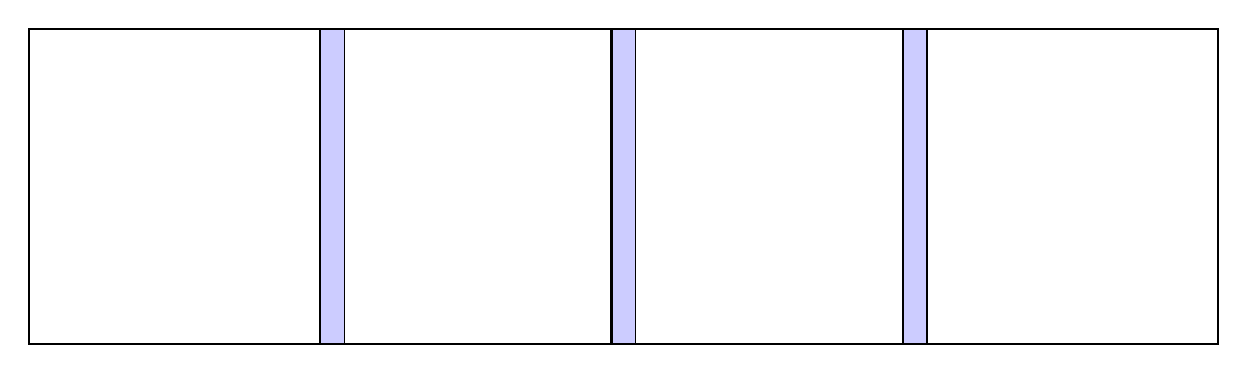
\begin{tikzpicture}

% Parameters
\def\squareSize{4}         % Width and height of each square
\def\overlap{0.3}          % Overlap amount (5% of 4 units = 0.3)

% Draw squares and overlaps
\foreach \i in {0,1,2,3} {
    \pgfmathsetmacro\xshift{\i*(\squareSize - \overlap)}
    \draw[thick] (\xshift,0) rectangle ++(\squareSize,\squareSize);
    
    % Draw overlapping region (except after last square)
    \ifnum\i<3
        \pgfmathsetmacro\xoverlap{\xshift + \squareSize - \overlap}
        \fill[blue!20] (\xoverlap,0) rectangle ++(\overlap,\squareSize);
    \fi
}

\end{tikzpicture}

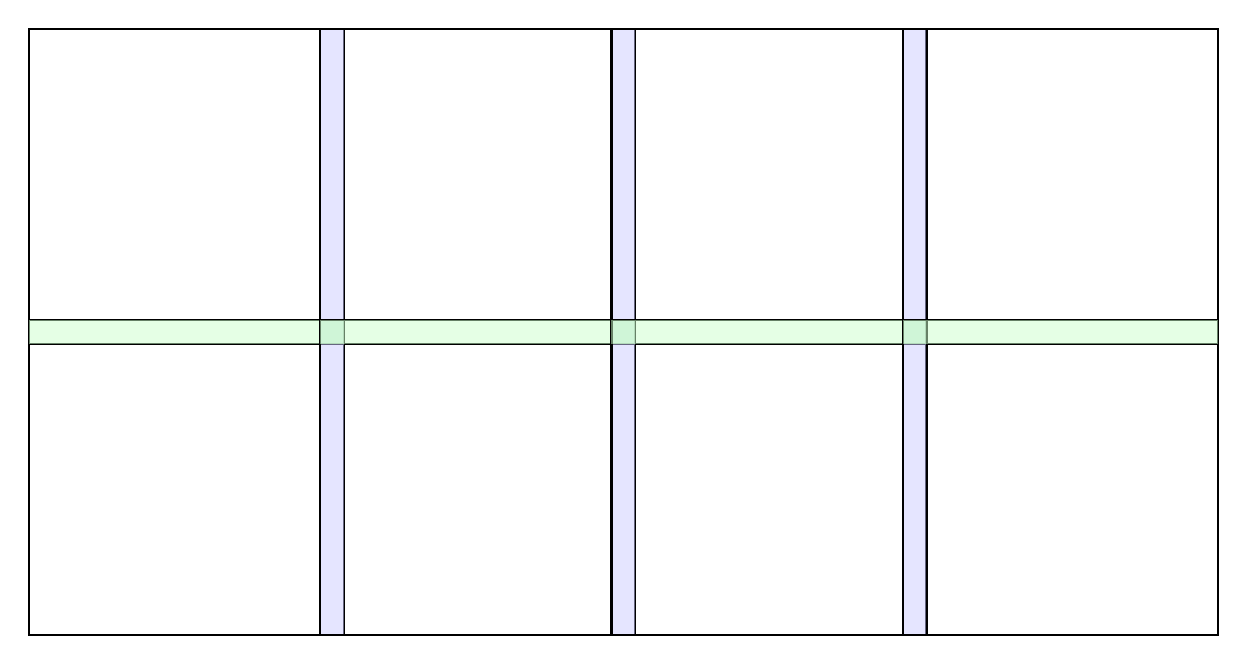
\begin{tikzpicture}

% Parameters
\def\squareSize{4}         % Width and height of each square
\def\overlap{0.3}          % Overlap amount (7.5% of 4 units = 0.3)
\def\rowGap{0.3}           % Vertical overlap between rows

% Draw top and bottom rows
\foreach \row in {0,1} {
    \foreach \i in {0,1,2,3} {
        \pgfmathsetmacro\xshift{\i*(\squareSize - \overlap)}
        \pgfmathsetmacro\yshift{-\row*(\squareSize - \rowGap)}
        
        % Draw the square
        \draw[thick] (\xshift,\yshift) rectangle ++(\squareSize,\squareSize);
        
        % Horizontal overlap (to the right), only for first 3 squares
        \ifnum\i<3
            \pgfmathsetmacro\xoverlap{\xshift + \squareSize - \overlap}
            \fill[blue!20, opacity=0.5] (\xoverlap,\yshift) rectangle ++(\overlap,\squareSize);
        \fi
        
        % Vertical overlap (with the row above), only for bottom row
        \ifnum\row=1
            \fill[green!20, opacity=.5] (\xshift,\yshift + \squareSize - \rowGap)
                rectangle ++(\squareSize,\rowGap);
        \fi
    }
}

\end{tikzpicture}